\documentclass[11pt, oneside]{article} 
\usepackage{geometry}
\geometry{letterpaper} 
\usepackage{graphicx}
	
\usepackage{amssymb}
\usepackage{amsmath}
\usepackage{parskip}
\usepackage{color}
\usepackage{hyperref}

\graphicspath{{/Users/telliott_admin/Dropbox/Tex/png/}}
% \begin{center} 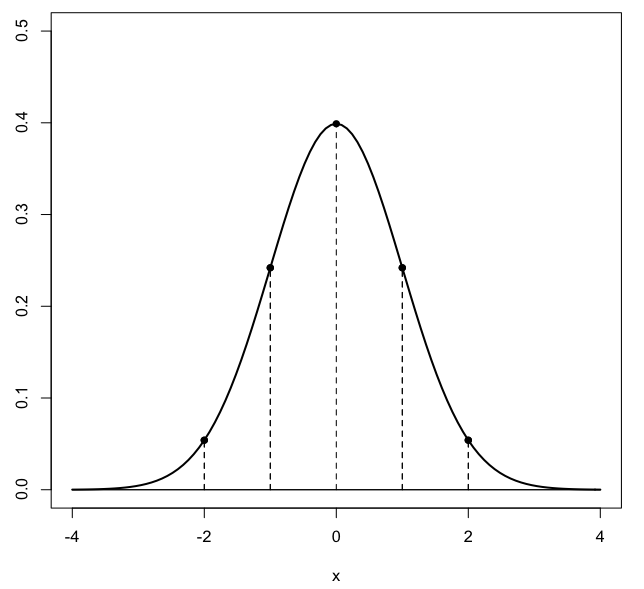
\includegraphics [scale=0.4] {gauss3.png} \end{center}

\title{Mean Value Theorem}
\date{}

\begin{document}
\maketitle
\Large


A man passes a police car at point $A$ doing 60 mph (the speed limit) and 4 minutes later passes another police car at point $B$, also doing 60 mph, yet the second officer writes him a ticket for speeding, justified by the mean value theorem.  

The reason:  point $A$ and point $B$ are 5 miles apart, hence the average speed over this interval was 75 mph, and \emph{must at least have been equaled at some point}.

If $f$ is a "nice" function on the interval $(a,b)$ then there exists at least one point $c$ in that interval where
\[ f'(c) = \frac{f(b) - f(a)}{b-a} \]
\begin{center} 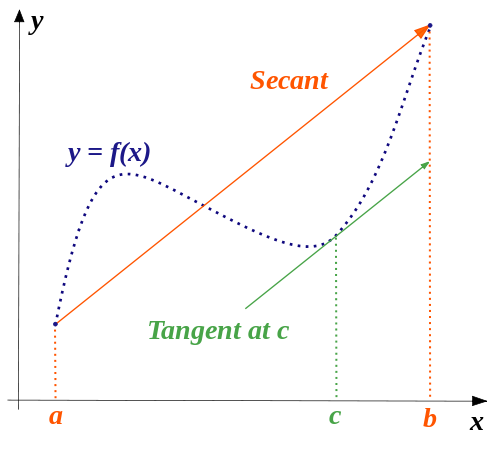
\includegraphics [scale=0.4] {mvt.png} \end{center}

What does it take to be "nice"?  The function $f$ must be continuous over the closed interval $[a,b]$ and differentiable over the open interval $(a,b)$.

The proof of the MVT relies on Rolle's Theorem, which is similar.  Rolle's Theorem says that for a "nice" $f$, if $f(a) = f(b)$, then there will exist at least one point $c$ in the interval $(a,b)$ such that $f'(c) = 0$.  

The MVT proof basically turns Rolle's interval so that $f(a) = f(b)$.

\subsection*{Proof}
We construct a new function utilizing the slope of the line connecting $a$ and $b$.  That slope is
\[ m = \frac{f(b) - f(a)}{b - a} \]

The equation of the line connecting the two endpoints is
\[ m(x-a) + f(a) \]

We subtract the above from $f(x)$ to construct our new function.  This is what "turns" $f(x)$ so the values at the endpoints are equal.  If we write it out in full:
\[ g(x) = f(x) - \ [ \ f(a) + \frac{f(b) - f(a)}{b - a}  \ (x-a) \ ] \]

Notice that at $x = a$ the term with $(x-a)$ is just zero so $g(a) = f(a) - f(a) = 0$.

On the other hand, at $x = b$ we have $g(b) = f(b) - f(a) - f(b) + f(a) = 0$.  Since $g(a) = g(b)$, Rolle's theorem applies.

What is the derivative of $g$?  To make life easier remember that the slope
\[ m = \frac{f(b) - f(a)}{b - a} \]
is \emph{just a number} and so is $f(a)$.  Hence

\[ g(x) = f(x) - \ [ \ f(a) + m(x-a) \ ] \]
\[ g'(x) = f'(x) - m \]
Rolle's theorem says that there is at least one value $x = c$ where this expression is zero, which means at that point:
\[ f'(c) = m = \frac{f(b) - f(a)}{b - a} \]
This completes the proof of the MVT.

\end{document}  